\subsection{Speaker Control}

The movement of the speaker is controlled by two servo motors which are connected to the GPIO Pins of the Raspberry Pi. The GPIO Pins can be controlled in Python using the \textbf{GPIOZero} library\cite{nuttall_gpio_2021} . It provides a class \lstpython{servo} which takes the pin to which the servo is connected. The servo can then be positoned by setting \lstpython{servo.value} to a value between $0$ and $1$. Note that \lstpython{servo} works with every pin but just pin \textbf{12} and \textbf{13} support hardware PWM. For the other pins the PWM will be created by software. This variant usually generates some jitter which makes the servo tremble. To make sure the hardware PWM is used for pin \textbf{12} and \textbf{13} the pin factory should be changed to \lstpython{PiGPIOFactory} (Listing \ref{lst:software:mov:pin_factory}).\cite{nuttall_gpio_2021}
%
\begin{mdframed}
\begin{lstlisting}[language=Python, caption=Changing the pin factory, label=lst:software:mov:pin_factory]
from gpiozero.pins.pigpio import PiGPIOFactory
from gpiozero import Device
Device.pin_factory = PiGPIOFactory()
\end{lstlisting}
\end{mdframed}
%
The configuration and control of the servo is handled in the HAL class \lstpython{ServoHAL} (Listing \ref{lst:software:mov:servo}). The class provides options to invert the servo or set an offset if the servo arm is not centered properly. \lstpython{set_position()} takes an angle between $-90^\circ$ and $90^\circ$ and sets the servo position accordingly.
%
\begin{mdframed}
\begin{lstlisting}[language=Python, caption=Servo configuration and control, label=lst:software:mov:servo]
class ServoHAL(HAL):

def __init__(self, pin: int, inverted: bool, offset: float):
    self.pin = pin
    self.offset = offset
    self.inverted = -1 if inverted else 1

    self.pwm = Servo(pin, initial_value=self._map_position(0), min_pulse_width=0.615 /
                      1000, max_pulse_width=2.495 / 1000)

def _map_position(self, angle: float):
    pos = self.inverted * (angle + self.offset) / 90

    if pos > 1: pos = 1
    if pos < -1: pos = -1

    return pos

def set_position(self, pos: float):
    self.pwm.value = self._map_position(pos)

def close(self):
    self.pwm.value = None
\end{lstlisting}
\end{mdframed}
%
In the class \lstpython{SpeakerControl} the \lstpython{ServoHAL} class is used to actually tilt the speaker. The class defines two servos for rotation around the x- and y-axis. Tilting can be initiated using the \lstpython{tilt_x()} or \lstpython{tilt_y()} method one of which is shown in listing \ref{lst:software:mov:tilt}. Both methods take the tilting angle in degree an map it to the corresponding servo postion using \lstpython{_map_position()} which implements the calculations from section \secref{sec:const:tilt}. The result is used to change the servo position.
%
\begin{mdframed}
\begin{lstlisting}[language=python, caption=Method for titling the speaker around the x-axis, label=lst:software:mov:tilt]
def tilt_x(self, angle: float):
  servo_pos = self._map_position(angle)

  print(f"Tilt X - {servo_pos}")

  self._x_servo.set_position(servo_pos)
  self.x_angle = angle
\end{lstlisting}
\end{mdframed}

\subsection{Control Interface}
%
The control interface consists of a website where a user can set the tilting angle of the speaker and an API over which the speaker is actually controlled. Both are created in Python with the \textbf{aiohttp} library.\cite{noauthor_aiohttp_nodate}

\subsubsection*{API}

The API is generated in the class \lstpython{API}. It registers the routes \textit{tilt/x}, \textit{tilt/y} and \textit{tilt} as shown in listing \ref{lst:software:mov:api}.
\textit{tilt/x} and \textit{tilt/y} are used to post a new titling angle to the server. \textit{tilt} returns the current tilting position around the x- and y-axis in JSON format.
%
\begin{mdframed}
\begin{lstlisting}[language=Python, caption=Control interface API, label=lst:software:mov:api]
class API:
  def __init__(self, server: web.Application) -> None:
      self.server = server
      self._create_api()

  def _create_api(self):
      self.speaker_control = SpeakerControl(12, 13)
      self.server.router.add_post("/tilt/x", self._tilt_x_handler)
      self.server.router.add_post("/tilt/y", self._tilt_y_handler)
      self.server.router.add_get("/tilt", self._get_tilt_handler)

  async def _tilt_x_handler(self, req: web.Request):
      try:
          content = json.loads(await req.text())
          angle = content["value"]
          self.speaker_control.tilt_x(angle)

          res = dict(success=True, message="")
      except Exception as err:
          res = dict(success=True, message=getattr(
              err, "message", repr(err)))

      return web.Response(text=json.dumps(res), content_type='application/json')

  async def _tilt_y_handler(self, req: web.Request):
      try:
          content = json.loads(await req.text())
          angle = content["value"]
          self.speaker_control.tilt_y(angle)

          res = dict(success=True, message="")
      except Exception as err:
          res = dict(success=True, message=getattr(
              err, "message", repr(err)))

      return web.Response(text=json.dumps(res), content_type='application/json')

  async def _get_tilt_handler(self, req: web.Request):
      return web.Response(
          text=json.dumps(dict(
              x=self.speaker_control.x_angle,
              y=self.speaker_control.y_angle
          )), content_type='application/json')
\end{lstlisting}
\end{mdframed}

\subsubsection*{Website}

Even though the API can be used to control the speaker programmatically a website provides an easy interface for manual inputs.\p
%
In order to publish a website, a webserver needs to be configured. This is done in the class \lstpython{Webserver}. As shown in listing \ref{lst:software:mov:webserver} the constructor takes a reference to the \textbf{aiohttp} Application and a path to the directory containing the \textit{.html}, \textit{.js} and \textit{.css} files. The webserver checks all files contained in this directory and registers new routes for each file so they can be accessed from a webbrowser.
%
\begin{mdframed}
\begin{lstlisting}[language=Python, caption=Minimal python webserver, label=lst:software:mov:webserver]
class Webserver:
  def __init__(self, server: web.Application, web_directory: str) -> None:
      self.server = server
      self.web_path = web_directory
      self._create_webserver()

  def _create_webserver(self):
      files = os.listdir(self.web_path)
      routes = self._create_routes(files)
      for route in routes:
          self.server.router.add_get(f"/{route}", self._webadress_handler)

      self.web_routes = routes

  async def _webadress_handler(self, req: web.Request):
      path = req.path.lstrip("/")
      route_config = self.web_routes[path]
      with open(os.path.join(self.web_path, route_config[0])) as f:
          return web.Response(text=f.read(), content_type=route_config[1])

  def _create_routes(self, files: List[str]) -> Dict[str, Tuple[str, str]]:
      routes = {}
      for file in files:
          route = file
          split_file = os.path.splitext(file)
          content_type = f"text/{split_file[1].lstrip('.')}"
          if split_file[1] == ".html":
              if split_file[0] == "index":
                  route = ""
              else:
                  route = f"{split_file[0]}"
          if split_file[1] == ".js":
              content_type == f"text/javascript"

          routes[route] = (file, content_type)

      return routes
\end{lstlisting}
\end{mdframed}
%
\newpage\noindent
The design of the website is shown in figure \ref{fig:software:mov:website}. When the site is loaded it uses the \textit{tilt} route to get the current position of the speaker. Now the two text fields can be used to enter a new angle for rotation around the x- or y-axis. Clicking on the \textbf{move} button will post this input to \textit{tilt/x} and \textit{tilt/y} respectively.
%
\begin{figure}[ht]
  \centering
  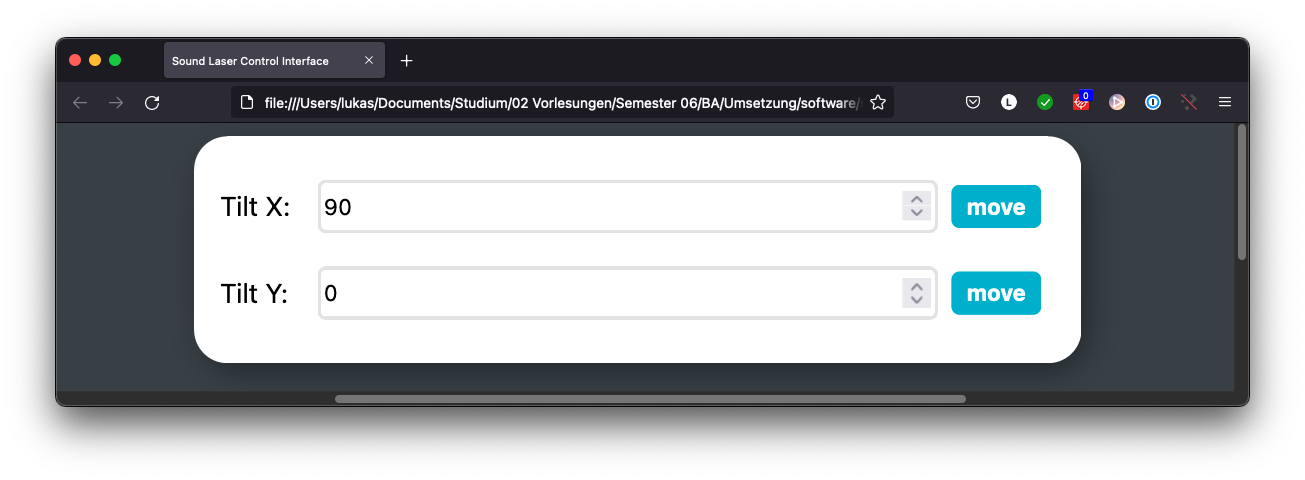
\includegraphics[height=\smallheight]{src/assets/pictures/software/control_interface_xl.png}
  \caption{Graphical control interface of the speaker}\label{fig:software:mov:website}
\end{figure}